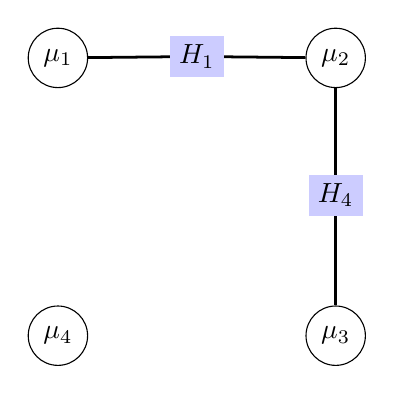
\begin{tikzpicture}[scale=.5]
\node (H1) at (225bp,-125bp)[draw,circle,fill=white] {$\mu_1$};
\node (H2) at (425bp,-125bp)[draw,circle,fill=white] {$\mu_2$};
\node (H3) at (425bp,-325bp)[draw,circle,fill=white] {$\mu_3$};
\node (H4) at (225bp,-325bp)[draw,circle,fill=white] {$\mu_4$};
\draw [line width=1pt] (H1) to (325bp, -124bp) node[fill=blue!20] {$H_{1}$} to (H2);
\draw [line width=1pt] (H2) to (425bp, -224bp) node[fill=blue!20] {$H_{4}$} to (H3);
\end{tikzpicture}
